\documentclass{article}
\usepackage{amsmath}

\usepackage{pgfplots}
\usepackage{tikz}
\usetikzlibrary{shapes, calc, scopes, decorations.pathmorphing,patterns}
\pgfplotsset{compat=1.15}

\usepackage{fancyhdr}
\usepackage[a4paper,left=1in,right=1in,top=1.5in,bottom=1in]{geometry} % Uncomment for narrow margins
\usepackage{parskip}
\usepackage{float}

\date{x/x/20xx}
\newcommand\addtag{\refstepcounter{equation}\tag{\theequation}}
\renewcommand*{\arraystretch}{1.5}

\def\iangle{35}


\begin{document}

\fancyhead[R]{PAT Guideline}
\pagestyle{fancy}


\section{Overview}
\subsection{Mathematics}

\textbf{Geometry.} Basic triangle and circular geometry. Polygons. Trigonometry. \textbf{Probability.} Conditional probability. Basic combinatorics. \textbf{Polynomials.} Factorisation, quadratic solutions and binomial expansion. \textbf{Functions.} Graph sketching and inequalities. \textbf{Algebra.} Solving trigonometric equations and manipulation of logarithmic and exponential equations. \textbf{Series.} Arithmetic and geometric series.

\textbf{Calculus.} Differentiation. Identifying and classifying turning points using differentiation. Integration and using it to find the area under a curve. Integration of fractions of polynomials.

\subsection{Physics}

\textbf{Linear mechanics.} Application of Newton's laws to basic mechanics problems. Analysis of pulleys, levers and other elementary systems. Springs and Hooke's law. Basic treatment of simple harmonic motion. Interpretation of graphs. Conservation of energy and momentum. Power and work. \textbf{Circular motion.} Centripetal force and angular velocity. Period of rotation.

\textbf{Waves.} Longitudinal and transverse waves. Properties of a plane wave: amplitude, frequency, period, wavelength and speed. Stationary waves. \textbf{Optics.} Refraction. Snell's law and application to prisms and optical fibres. Total internal reflection. Elementary treatment of single and double slit diffraction.

\textbf{Electromagnetism.} Coulomb forces. Force under an electric field. Magnetic fields. Application to transformers. \textbf{Circuits.} Parallel and series circuits. Current as a flow of electrons. Properties of elementary circuit components including filament lamps, diodes, capacitors, light-dependent resistors and thermistors. \textbf{Photoelectric effect.} Work function. Energy of accelerated electron beams. \textbf{Radiation.} Power law.

\textbf{Gravity.} Newtonian gravity and circular orbits. Geostationary and polar orbits. Properties of the solar system. \textbf{Atomic structure.} Energy levels. \textbf{Nuclear.} Decays. Half-life.


\section{Mathematics}

\subsection{Geometry}

\textbf{Triangle geometry.} Similar triangles. A triangle with two sides of same length is an isosceles. If $a=b$ below, then $\alpha=\beta$.
\begin{figure}[h]
\centering
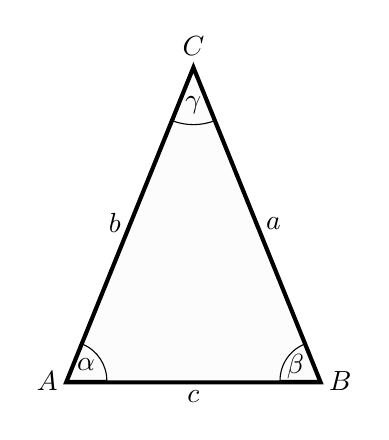
\begin{tikzpicture}
    \node[isosceles triangle, isosceles triangle apex angle=44,draw,
        inner sep=0pt,anchor=lower side,rotate=90,draw=black,
        line width=1.5pt, minimum height=4cm, fill=gray!2] (triangle) at (1.6,-0.05) {};
        
    \draw (0,0) -- (0:0.50cm) arc (0:68:.50cm);
    \begin{scope}[shift={(3.2cm,0cm)}]
        \draw (0,0) -- (-180:0.50cm) arc (180:110:0.5cm);
        \draw (150:0.35cm) node {$\beta$};
    \end{scope}

    \begin{scope}[shift={(1.6cm,4cm)}]
        \draw (0,0) -- (250:.75cm) arc (250:292:.75cm);
        \draw (-90:0.5cm) node {$\gamma$};
    \end{scope}

    \coordinate[label=left:$A$] (A) at (0,0);
    \coordinate[label=right:$B$] (B) at (3.2,0);
    \coordinate[label=above:$C$] (C) at (1.6,4);

    \coordinate[label=below:$c$](c) at ($ (A)!.5!(B) $);
    \coordinate[label=left:$b$](b) at ($ (A)!.5!(C) $);
    \coordinate[label=right:$a$](a) at ($ (B)!.5!(C) $);
    
    \coordinate[label=45:$\alpha$] (Alpha) at (A);
\end{tikzpicture}
\end{figure}

\textbf{Sine rule.}
\[
\frac{a}{\sin\alpha}=\frac{b}{\sin\beta}=\frac{c}{\sin\gamma}
\]
\textbf{Cosine rule.}
\[
c^2=a^2+b^2-2ab\cos\gamma
\]

\textbf{Circular geometry.} The tangent to a circle at point $p$ on the circle is perpendicular to the line passing through the radius and the point $p$.

\textbf{Polygons.} An $N$-gon has an exterior angle of $360^\circ / N$. Its interior angle is $180^\circ - 360^\circ/N$.

\subsection{Probability}

The probability of an observed event $A$ out of the total possible outcomes $\Omega$ is given by 
\[
P(A)=\frac{|A|}{|\Omega|}\,,
\]
where $|A|$ is the size of the set $A$.

\textbf{Conditional probability.} The probability of an event $A$ given $B$ is
\[
P(A|B)=\frac{P(A\cap B)}{P(B)}\,.
\]
It can be interpreted as the probability of observing $A$ given that we have previously observed $B$. For example the probability of getting all tails on three throws of a fair coin given that one of the throws is a tail is $\frac{1}{7}$, since there are 7 outcomes in the three throws with at least one tail, and there is only 1 outcome where all of them are tails.

\textbf{Combinatorics.} The number of ways of ordering a set with $N$ elements is $N!$. The number of ways of picking $r$ elements out of a set of $N$ elements is $\binom{N}{r}$, where
\[
\binom{N}{r}=\frac{N!}{r!(N-r)!}\,.
\]
In general if we have $r$ choices and $m_i$ possibilities in the $i$th choice, then the total number of different possibilities is $\prod_{i=1}^rm_i$.

\subsection{Polynomials}

An $N$th-order polynomial has at most $N$ roots. If $\{x_0,x_1,\ldots,x_N\}$ denote the set of roots for a polynomial $a+bx+cx^2+dx^3+\ldots+x^N$, then it can be written as
\[
a+bx+cx^2+dx^3+\ldots+x^N = (x-x_0)(x-x_1)(x-x_2)\ldots(x-x_N)\,.
\]
The binomial expansion is given by
\begin{align*}
(x+a)^n &= x^n + \binom{n}{1} x^{n-1} a + \binom{n}{2} x^{n-2} a^2 + \ldots + a^n\\
&= x^n + n x^{n-1}a+\frac{n(n-1)}{2!} x^{n-2}a^2 + \frac{n(n-1)(n-2)}{3!}x^{n-3} a^3 + \ldots + a^n
\end{align*}

\subsection{Graph sketching}
Checklist for graph sketching:
\begin{enumerate}
    \item Compute values of $(x,y)$ when $x=0$, or when $y=0$, if it exists. Look at ``special" points such as $x=1$ and $x=1/2$ in the function
    \[
    y=e^{2(x-1)} + e^{4x-2}\,.
    \]
    \item Look for asymptotic values, if any. If $x=a$ is an asymptotic value, look at the sign of $y(a^+)$ and $y(a^-)$ to determine the sign of the infinity at $y(a)$.
    \item Find limit points of $y$, i.e. compute $y$ when $x\rightarrow\pm\infty$.
    \item Find stationary points of the function.
\end{enumerate}
Remember to label all special points of the graph.

\textbf{Inequalities.} For any quadratic with roots $a$, $b$, $a > b$, the inequality
\[
(x-a)(x-b)>0
\]
has solutions $x>a$, $x<b$. Similarly the inequality
\[
(x-a)(x-b)<0
\]
has solutions $b<x<a$.

\subsection{Series}

\textbf{Arithmetic progression.} This is a sequence where the terms are separated by a constant gap, e.g. $2,5,8,11,14,\ldots$. The $n$th term is given by
\[
a_n = a_1 + (n-1)d\,,\qquad n=1,2,\ldots\,
\]
Its sum is
\[
\sum_{n=1}^N a_n = \frac{N(a_1+a_N)}{2}\,.
\]
\textbf{Geometric progression.} This has a general term of $a_n=a r^n$. Its sum is given by
\[
\sum_{n=0}^{N-1} ar^n = \frac{a(1-r^N)}{1-r}\,. 
\]
Taking $N\rightarrow\infty$, the sum converges if $|r|<1$, and we get
\[
\sum_{n=0}^\infty ar^n = \frac{a}{1-r}\,.
\]

\subsection{Calculus}

\textbf{Implicit differentiation.} Given a curve
\[
x^3+3x^2y^4+y^4 = 0\,,
\]
we can differentiate it with respect to $x$ using the product and chain rule:
\begin{align*}
    \frac{d}{dx}(3x^2y^4) &= y^4\frac{d}{dx}(3x^2) + 3x^2\frac{d}{dx}(y^4)\\
    &= 6xy^4 + 3x^2\frac{dy}{dx}\frac{d}{dy}(y^4)\\
    &= 6xy^4 + 12x^2y^3\frac{dy}{dx}\,.
\end{align*}
So we have
\begin{align*}
    \frac{d}{dx}(x^3+3x^2y^4+y^4)&=3x^2+6xy^4 + 12x^2y^3\frac{dy}{dx}+4y^3\frac{dy}{dx}\\
    &=0\,,
\end{align*}
which we can rearrange to find
\[
\frac{dy}{dx} = \frac{3x^2+6xy^4}{12x^2y^3+4y^3}\,.
\]
To find the gradient of this curve at a particular point, we simply substitute its $(x,y)$ value in the above expression, e.g. at $(2,1)$ we have
\[
\left.\frac{dy}{dx}\right|_{(2,1)} = \frac{3\cdot 4+6\cdot2}{12\cdot4+4} = \frac{24}{52} = \frac{6}{13}
\]

\textbf{Tangent and normal.} If $y=mx+c$ is the equation of the line tangent to a curve at point $(a,b)$, then
\[
m=\left.\frac{dy}{dx}\right|_{(a,b)}\,.
\]
We can then find $c$ by substituting the point $(a,b)$ back into the equation of the line.

If we want to find the equation of the normal instead, then the gradient of the line is $-\frac{1}{m}$.

\textbf{Turning points.} A turning point is a point $(x,y)$ where $dy/dx$ is zero. If $d^2y/dx^2 >0$, then this point is a minimum. If $d^2y/dx^2 <0$, this point is a maximum. If $d^2y/dx^2=0$, we call this point a \emph{point of inflection} and we cannot determine exactly whether it is a maximum or minimum (have to look at higher derivatives).

For example, $y=x^3$ has a point of inflection at $x=0$.
\begin{figure}[h]
    \centering
    \begin{tikzpicture}[scale=0.8]
        \begin{axis}[axis x line=middle, axis y line=middle, xmax = 3, xmin=-3, xtick={0}, ytick={0}]
            \addplot[color=blue,domain=-2.5:2.5] {x*x*x};
        \end{axis}
    \end{tikzpicture}
\end{figure}

\textbf{Integration.} The integration of a curve between two points $x=a$ and $x=b$ is the area between the curve and the $x$-axis within the two points. It will give a negative value if the curve is below the $x$-axis in that region.

The integration of a fraction whose numerator is the derivative of the denominator can be easily calculated. For example, consider the following integral:
\[
\int dx\frac{2x+6}{(x^2+6x+8)^\frac{3}{2}}\,.
\]
Let $y=x^2+6x+8$. Then we can substitute the numerator with $dy/dx$, which gives
\[
\int dx\frac{2x+6}{(x^2+6x+8)^\frac{3}{2}}=\int dx\left(\frac{dy}{dx}\right)\frac{1}{y^\frac{3}{2}}=\int \frac{dy}{y^\frac{3}{2}} = -\frac{2}{y^\frac{1}{2}} = -\frac{2}{(x^2+6x+8)^\frac{1}{2}}\,.
\]
If the numerator cannot be written as the derivative of the denominator, but the denominator is still a polynomial, we can factorise it and split it into several fractions. For example,
\[
\frac{1}{x^2+6x+8} = \frac{1}{(x+4)(x+2)} = \frac{A}{x+4} + \frac{B}{x+2}
\]
where $A$, $B$ are constants to be found. We solve them by equating the coefficients,
\begin{align*}
    \frac{1}{(x+4)(x+2)} &= \frac{A(x+2)+B(x+4)}{(x+2)(x+4)}\\
    &= \frac{(A+B)x+2A+4B}{(x+2)(x+4)}\,,
\end{align*}
so we have
\begin{align*}
    A+B&=0\\
    2A+4B&=1\,,
\end{align*}
which gives $A=-B$, $B=1/2$ so $A=-1/2$. So
\[
\int dx\frac{1}{(x+4)(x+2)} = \int dx\left(-\frac{1}{2(x+4)}+\frac{1}{2(x+2)}\right) = -\frac{1}{2}\ln(x+4)+\frac{1}{2}\ln(x+2)\,.
\]

\section{Physics}
\subsection{Linear mechanics}
\textbf{Velocity and acceleration.} If $x$ is the displacement or position of the particle at time $t$, then
\[
v=\frac{dx}{dt}\,,\qquad a=\frac{dv}{dt}=\frac{d^2x}{dt^2}\,.
\]
When $a$ is constant, one can use the ``suvat" equations. When $a=0$, $x=vt$.

\textbf{Block on a plane.} Identify the forces in a free body diagram and resolve them in the appropriate directions.
\begin{figure}[H]
    \centering
    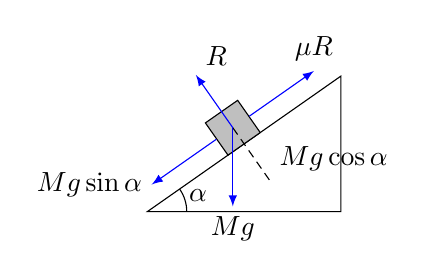
\begin{tikzpicture}[plane/.style={draw=black},
    M/.style={rectangle,draw,fill=lightgray,minimum size=0.5cm,thin},
    force/.style={>=latex,draw=blue,fill=blue}]
        \draw[plane] (0,-1) coordinate (base)
                     -- coordinate[pos=0.5] (mid) ++(\iangle:3) coordinate (top) |- (base) -- cycle;
        \path (mid) node[M,rotate=\iangle,yshift=0.25cm] (M) {};
        \draw[-] (base)++(0.5cm,0) arc (0:\iangle:0.5cm);
        \path (base)++(\iangle*0.5:0.5cm+5pt) node {$\alpha$};
        \begin{scope}[rotate=\iangle]
            \draw[densely dashed] (M.center) -- ++(0,{-cos(\iangle)}) node[above right] {$Mg\cos\alpha$};
        
            {[force,->]
                \draw (M.west) -- ++(-1,0) node[left] {$Mg\sin\alpha$};
                \draw (M.east) -- ++(1,0) node[above] {$\mu R$};
                \draw (M.center) -- ++(0,{cos(\iangle)}) node[above right] {$R$};
            }
        \end{scope}
        \draw[force,->] (M.center) -- ++(0,-1) node[below] {$Mg$};
    \end{tikzpicture}
\end{figure}

\textbf{Pulleys.} The tension on each of the strings on the pulley are the same.

\def\arcr{0.5cm}
\begin{figure}[H]
    \centering
    \begin{tikzpicture}[
        force/.style={>=latex,draw=blue,fill=blue},
        axis/.style={densely dashed,gray,font=\small},
        M/.style={rectangle,draw,fill=lightgray,minimum size=0.5cm,thin},
        m/.style={rectangle,draw=black,fill=lightgray,minimum size=0.3cm,thin},
        plane/.style={draw=black},
        string/.style={draw=red, thick},
        pulley/.style={thick},
    ]
    
        \draw[plane] (0,-1) coordinate (base)
                     -- coordinate[pos=0.5] (mid) ++(\iangle:3) coordinate (top)
                     |- (base) -- cycle;
        \path (mid) node[M,rotate=\iangle,yshift=0.25cm] (M) {};
        \draw[pulley] (top) -- ++(\iangle:0.25) circle (0.25cm)
                       ++ (90-\iangle:0.5) coordinate (pulley);
        \draw[string] (M.east) -- node[above] {$T$} ++(\iangle:1.5cm)  arc (90+\iangle:0:0.25) -- node[right] {$T$} ++(0,-1) node[m] (m) {};
    
        \draw[-] (base)++(\arcr,0) arc (0:\iangle:\arcr);
        \path (base)++(\iangle*0.5:\arcr+5pt) node {$\alpha$};
        \draw[force,->] (M.center) -- ++(0,-1) node[below] {$Mg$};
        \draw[force,->] (m.center) -- ++(0,-1) node[below] {$mg$};
    \end{tikzpicture}
\end{figure}

Make sure to choose a consistent direction for the acceleration before writing down the equation of motion for both blocks. For example, if $a$ is pointing downwards from the small block, then we have
\begin{align*}
    ma &= mg -T\\
    Ma &= T - Mg\sin\alpha
\end{align*}

\textbf{Hooke's law.} The force from a spring with spring constant $k$ is given by $F=-kx$, where $x$ is the extension of the spring from its natural length.

For two springs connected in series with spring constants $k_1$, $k_2$, its combined effective spring constant is
\[
\frac{1}{k_{\text{eff}}}=\frac{1}{k_1}+\frac{1}{k_2}\,.
\]
This is because the force from the two springs have to be equal,
\[
F=k_1x_1=k_2x_2\Rightarrow x_2=\frac{k_1}{k_2}x_1\,,
\]
and we want to find $k_\text{eff}$ in $F=-k_\text{eff}(x_1+x_2)$.

For two springs connected in parallel, with equal natural length, the effective spring constant is simply $k_\text{eff}=k_1+k_2$.

The potential energy of a spring extended a distance $x$ from its natural length is $E=\frac{1}{2}kx^2$.

\textbf{Simple harmonic motion.} Whenever we have a force (or acceleration) that is proportional to the opposite direction of displacement, $F\propto -x$, we have simple harmonic motion. This is an oscillatory movement with a period $T$ and amplitude $A$.

Suppose we have $F=-\alpha x$. Then the angular frequency $\omega$ of oscillation is given by
\[
a=-\omega^2x\Rightarrow\omega^2=\frac{\alpha}{m}\,.
\]
We can then find $T$ using $\omega=2\pi/T$. The amplitude is then equal to the initial displacement $x_0$ about the equilibrium point.
\begin{figure}[h]
    \centering
    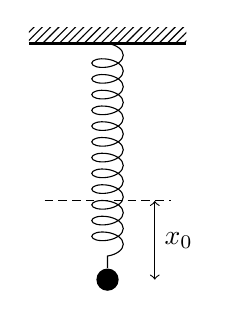
\begin{tikzpicture}
        \node[circle, fill=black, inner sep=1mm] (a) at (0,0) {};
        \draw[decoration={aspect=0.5, segment length=2mm, amplitude=2mm,coil},decorate] (0,3) -- (a);
        
        \fill [pattern = north east lines] (-1,3) rectangle (1,3.2);
        \draw[thick] (-1,3) -- (1,3);
        \draw[densely dashed] (-0.8,1) -- (0.8,1);
        \draw[<->] (0.6,1)--node[right]{$x_0$} (0.6,0);
    \end{tikzpicture}
\end{figure}

\textbf{Graphs.} From the calculus forms of the velocity and acceleration, the total displacement in a velocity-time graph is the area under the velocity curve, i.e. the integration of the velocity.
\[
\int_{x=x_0}^x dx =\int_{t=0}^tvdt
\]
The velocity (or acceleration) may be represented as a function of displacement as well, which in this case the total displacement is \textbf{not} the area underneath the curve.

The work done in a force-distance graph is given by the area underneath the force curve, since
\[
W=\int F(x)dx\,.
\]
Similarly energy and power are related by
\[
E=\int P(t)dt\,.
\]

\textbf{Energy and momentum.} Energy is composed of two parts: kinetic energy and the potential energy. The potential energy is the work done needed to place the particle in the potential. For example in gravity we have
\[
E=\frac{1}{2}mv^2-\frac{GMm}{r}\,.
\]
The total energy is conserved. This means that it does not change over time.

The total momentum is the sum of each particle's momenta, taking into account its direction. For example two particles travelling towards each other with speed $v_1$, $v_2$ has total momentum $P=m_1v_1-m_2v_2$ (in the direction of $v_1$). The total momentum is conserved as long as there are no frictional or drag forces.

\textbf{Circular motion.} The angular velocity $\omega$ is the change in $\theta$ over time. For circular motion, we have
\[
\theta=\omega t\,,\qquad\omega=\frac{v}{r}\,,\qquad a=\frac{v^2}{r}=\omega^2r\,,\qquad \omega=\frac{2\pi}{T}\,,
\]
where $T$ is the period of rotation. The force on a particle in circular motion is always perpendicular to its velocity. The force required to keep this particle in circular motion is called the centripetal force, $F=mv^2/r = m\omega^2r$.

For example a satellite in circular motion has its centripetal force equal to the gravitational force,
\[
\frac{mv^2}{r}=\frac{GMm}{r^2}\,.
\]

\subsection{Waves}

\textbf{Plane waves.} The amplitude and frequency of a plane wave are independent. We have the following relations:
\[
f=\frac{1}{T}\,,\qquad\omega=2\pi f\,,\qquad c=f\lambda\,.
\]
The power transmitted by the wave is proportional to the square of the amplitude.

\textbf{Stationary waves.} A plane wave propagating towards a wall perpendicular to the direction of propagation will set up a stationary wave.

A stationary wave has its maxima and minima fixed in time. The distance between consecutive maxima is $\lambda/2$, where $\lambda$ is the wavelength of the plane wave. The distance between a maximum and its adjacent minimum is $\lambda/4$.

\subsection{Optics}
\textbf{Refraction and Snell's law.} For light propagating from a medium with refractive index $n_1$ to another with $n_2$, the angles $\theta_1$, $\theta_2$ measured from the normal to the surface is given by
\[
n_1\sin\theta_1=n_2\sin\theta_2\,.
\]
Air and vacuum has a refractive index of $n=1$.
Total internal reflection occurs when the incoming angle is large enough. The critical angle is the incoming angle where the outgoing angle is at $90^\circ$. So a beam travelling inside a glass with refractive index $n$ should have an angle of $\theta\geq\theta_c$ where
\[
n\sin\theta_c=1\,.
\]
\textbf{Diffraction.} Single-slit diffraction has an angular spread of
\[
\theta\sim\frac{\lambda}{a}
\]
where $a$ is the width of the slit. No fringes are observed.
Double-slit diffraction gives fringes with separation 
\[
\Delta y=\frac{\lambda d}{a}\,,
\]
where $d$ is the distance from the slit to the screen. The fringes look like
\begin{figure}[H]
\centering
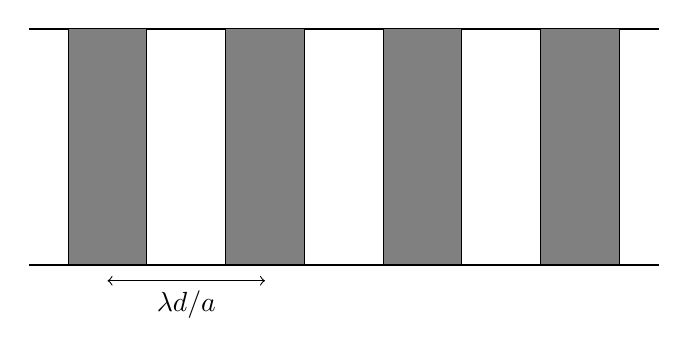
\begin{tikzpicture}
    \draw[thick] (-4,0)--(4,0);
    \draw[thick] (-4,3)--(4,3);
    \draw[fill=gray] (-2.5,0) rectangle (-3.5,3);
    \draw[fill=gray] (-1.5,0) rectangle (-0.5,3);
    \draw[fill=gray] (0.5,0) rectangle (1.5,3);
    \draw[fill=gray] (2.5,0) rectangle (3.5,3);
    \draw[<->] (-3,-0.2) -- node[below] {$\lambda d/a$} (-1,-0.2);
\end{tikzpicture}
\end{figure}

\subsection{Electromagnetism}

\textbf{Coulomb force.} For two charges $Q_1$, $Q_2$ separated by a distance $d$. The force felt by one due to the other is given by
\[
F=\frac{Q_1Q_2}{4\pi\varepsilon_0d^2}\,.
\]
The direction of this force is important. Remember that opposite charges attract, like charges repel.

\textbf{Electric and magnetic fields.} The force on a charge $q$ due to a constant electric field $E$ is given by $F=qE$. The constant electric field generated by two plates separated by a distance $d$ with a potential difference $V$ is $E=V/d$.

Magnetic field lines always form closed loops. A charged particle travelling in a purely magnetic field does not gain any energy. Thus the magnetic field does no work.

The potential difference induced on a wire from a time-varying magnetic field is given by Faraday's law,
\[
V=-NA\frac{d(B)}{dt}\,,
\]
where $A$ is the area that the field lines intersect with and $N$ the number of loops in the wire.

\textbf{Transformers.} A transformer works by placing two solenoids of different loop count near each other. AC current is passed through which generates a time-varying magnetic field. This induces a current on the other solenoid with a different potential difference. Using Faraday's law, we have
\[
\frac{V_1}{V_2} = \frac{N_1}{N_2} = \frac{I_2}{I_1}\,.
\]

\subsection{Circuits} The current is the charge flowing through the wire per unit time. It can be written as $I=dQ/dt$.

\textbf{Diodes.} These restrict the flow of current to one direction. For a diode pointing in the positive $V$ direction, it has a current-voltage graph of
\begin{figure}[H]
    \centering
    \begin{tikzpicture}[scale=0.7]
        \begin{axis}[axis x line = middle, axis y line=middle, xtick={-1.2,1.2}, ytick={0}, xlabel = $V$, ylabel = $I$, xticklabels={-0.6,0.6}]
            \addplot[color=blue,domain = -5:5] {x^3};
        \end{axis}
    \end{tikzpicture}
\end{figure}
The graph shows that $V\sim0.6$ is the minimum voltage for current to flow through. As $V<-0.6$ there is a breakdown and the diode allows current to go through.

\textbf{Capacitors.} Capacitors store charge at a certain voltage. The capacitance $C=Q/V$. The energy stored in a capacitor is
\[
E=\frac{1}{2}CV^2 = \frac{1}{2}QV = \frac{1}{2}\frac{Q^2}{C}\,.
\]
As the capacitor charges, the voltage approaches its specified voltage and the current drops down. All the curves are exponential in behaviour. The following graph is of a capacitor in series with a resistor with resistance $R$ being charged.
\begin{figure}[H]
    \centering
    \begin{tikzpicture}[scale=0.6]
        \matrix[column sep=1cm]{
            \begin{axis}[axis x line = middle, axis y line=middle, xtick={1}, ytick={1}, xlabel = $t$, ylabel = $I$, yticklabels={$I_0$}, xticklabels={$RC$}, ymax = 1.2, width=7cm, height=5cm]
            \addplot[color=blue,domain = 0:3] {exp(-x)};
            \end{axis}
        &
            \begin{axis}[axis x line = middle, axis y line=middle, xtick={1}, ytick={1}, xlabel = $t$, ylabel = $V$, yticklabels={$V_0$}, xticklabels={$RC$}, ymax = 1.2, width=7cm, height = 5cm]
            \addplot[color=blue,domain = 0:3] {1-exp(-x)};
            \end{axis}
        \\
        };
        
    \end{tikzpicture}
\end{figure}
The rate of current decay is $\tau=RC$, a quantity known as the time constant. When $t>\tau$, we can take $I$ to be roughly flattened out.

When the capacitor discharges, the current graph looks the same while the voltage graph is reversed: it starts from $V_0$ and decays to zero.

\textbf{Light-dependent resistor.} The LDR decreases with resistance as light intensity increases. The curve looks look an exponential decay.

\textbf{Resistance and temperature.}
\begin{figure}[H]
    \centering
    \begin{tikzpicture}
        \matrix[column sep=1cm]{
            \begin{axis}[axis x line = middle, axis y line=middle, xtick={0}, ytick={0}, xlabel=Wire, ylabel=$R$, width=6cm, height=5cm]
            \addplot[color=blue,domain = 0:3] {x/2.0+2};
            \end{axis}
        &
            \begin{axis}[axis x line = middle, axis y line=middle, xtick={0}, ytick={0}, xlabel=Filament lamp,ylabel=$R$, width=6cm, height = 5cm]
            \addplot[color=blue,domain = 0:3] {0.5+x^4};
            \end{axis}
        &
            \begin{axis}[axis x line = middle, axis y line=middle, xtick={0}, ytick={0}, xlabel=Thermistor,ylabel=$R$, width=6cm, height = 5cm]
            \addplot[color=blue,domain = 0:3] {exp(-x)};
            \end{axis}
        \\
        };
    \end{tikzpicture}
\end{figure}

\subsection{Photoelectric effect} The photoelectric effect is the emission of electrons from the surface of a metal due to incoming photons. The work function $\phi$ is the threshold energy of the photon energy needed to liberate an electron. Thus the kinetic energy of the electron is
\[
\text{KE}=\frac{hc}{\lambda} - \phi\,,
\]
where $\lambda$ is the wavelength of the photon.

A measure of electron energy is the electron volt (eV), where $1eV=1.6\times 10^{-19}J$. The kinetic energy of an electron accelerated under a potential difference $V_0$ is simply $eV_0$.

\subsection{Radiation}
Light radiated from a point source in all directions has a power drop proportional to $1/r^2$, i.e. $P\propto 1/r^2$.

\subsection{Gravity}
The force on a mass $m$ due to another mass $M$ a distance $d$ away is
\[
F=\frac{GMm}{d^2}\,.
\]
This force is always attractive. The gravitational potential from infinity to a point r from the mass is given by
\[
V=-\frac{GMm}{r}\,.
\]
This is negative as work is needed to bring a satellite out of the potential.

\textbf{Geostationary and polar orbits.} A geostationary orbit is where the satellite orbits at a fixed spot above the Earth (it always looks down at the same spot on the surface of the Earth). Thus it is always orbiting on the equator.

A polar orbit is where the satellite orbit passes through both poles.

\textbf{Circular orbit.} In a circular orbit, we have
\[
m\omega^2r=\frac{GMm}{r^2}\,.
\]
So we can relate the period of orbit $T$ to the radius,
\[
\left(\frac{2\pi}{T}\right)^2=\frac{GM}{r^3}\,,
\]
which gives $T^2\propto r^3$. This is known as Kepler's third law.

\subsection{Nuclear decay}
The equation of nuclear decay given a decay rate $\tau$ is
\[
N=N_0e^{-t/\tau}\,,
\]
where $N_0$ is the number of particles at time $t=0$. The half-life is the time $t_{1/2}$ when $N=N_0/2$ or
\[
\ln 2=\frac{t_{1/2}}{\tau}\,,
\]
so we have $\tau=t_{1/2}/\ln 2$.


\end{document}
